\documentclass[11pt,xcolor=table]{beamer}

\usetheme[progressbar=frametitle]{metropolis}
\usepackage{appendixnumberbeamer}
\usepackage{pgfpages}
%\setbeameroption{show notes on second screen}
  \setbeamertemplate{enumerate items}[square]
\usepackage{multirow}

\usepackage{graphicx}

\usepackage{xcolor}

\newcommand{\link}[3][mLightBrown]{\href{#2}{\color{#1}{#3}}}%


\newcommand{\questionslide}[0]{
{\setbeamercolor{palette primary}{fg=black, bg=yellow}
\begin{frame}[standout]
    \raggedright
  Any questions? \\ \vspace{1cm}
  \raggedleft
  \dots{ } Remember -- Every question is useful!
\end{frame}
}}

\newcommand{\task}[1]{
   \begin{alertblock}
   {\centering \vspace{-1.5ex} \\ #1  \\ \vspace{-1.5ex} }
   \end{alertblock}
   }

\setbeamercolor{block title alerted}{%
    use={block title, alerted text},
    bg=yellow,
    fg=black
}

\definecolor{peppermint}{RGB}{75, 161, 115}
%\definecolor{peppermint}{RGB}{75, 161, 115}


\setbeamercolor{alerted text}{fg=peppermint , bg= black}

\usepackage{booktabs}
\usepackage[scale=2]{ccicons}

\usepackage{pgfplots}
\usepgfplotslibrary{dateplot}

\makeatletter 
\def\beamer@framenotesbegin{% at beginning of slide
    \usebeamercolor[fg]{normal text}
    \gdef\beamer@noteitems{}% 
    \gdef\beamer@notes{}% 
}
\makeatother


\usepackage{xspace}
\newcommand{\themename}{\textbf{\textsc{metropolis}}\xspace}

\title{Semester Review, Questions, Exam Practice
}
\subtitle{Econ 140, Section 12}
% \date{\today}
\date{}
\author{Jonathan Old}

% \titlegraphic{\hfill\includegraphics[height=1.5cm]{logo.pdf}}

\begin{document}

\maketitle

\begin{frame}{Roadmap}
  \setbeamertemplate{section in toc}[sections numbered]
  \tableofcontents%[hideallsubsections]
\end{frame}





\begin{frame}{Course evaluation}
\centering

\includegraphics[width=0.6\textwidth]{figures/course_eval_qr.png}

   
\end{frame}



\section{Regression Discontinuity}



\begin{frame}{The world is full of arbitrary rules}
\begin{itemize}
    \item Students receive a scholarship if their GPA is above 3.0
    \item Children are allowed to start school if they are five years old before January 31 of that year
    \item Individuals are eligible for a microfinance loan if they own less than 0.5 acres of land
    \item Legislators are elected if they receive over 50\% of the vote
\end{itemize}

\alert{This creates wonderful discontinuities in the data that we can exploit for econometric analysis!} 

   
\end{frame}


\begin{frame}{The most important rules of regression discontinuity}

    \begin{itemize}
        \item The essence of RD is to compare people (units) just above the cut-off to others just below
        \item Crucial assumptions: There are no jumps but our jump at the jump // The effect of $X$ (our running variable) and any other variable $C$ on $Y$ (our outcome) is smooth around the discontinuity
        \item Identifying assumption: In the absence of the "treatment" (which was allocated by a discontinuous rule), the outcomes of the treated would have been essentially the same as the outcomes of the untreated
        \item Limitations: 
        \begin{enumerate}
            \item We only estimate a \textbf{local} effect!
            \item There may be strategic behavior at the cutoff (example: school district Oakland/Piedmont)
        \end{enumerate} 
        
    \end{itemize}
\end{frame}


\begin{frame}{Oakland and Piedmont }
    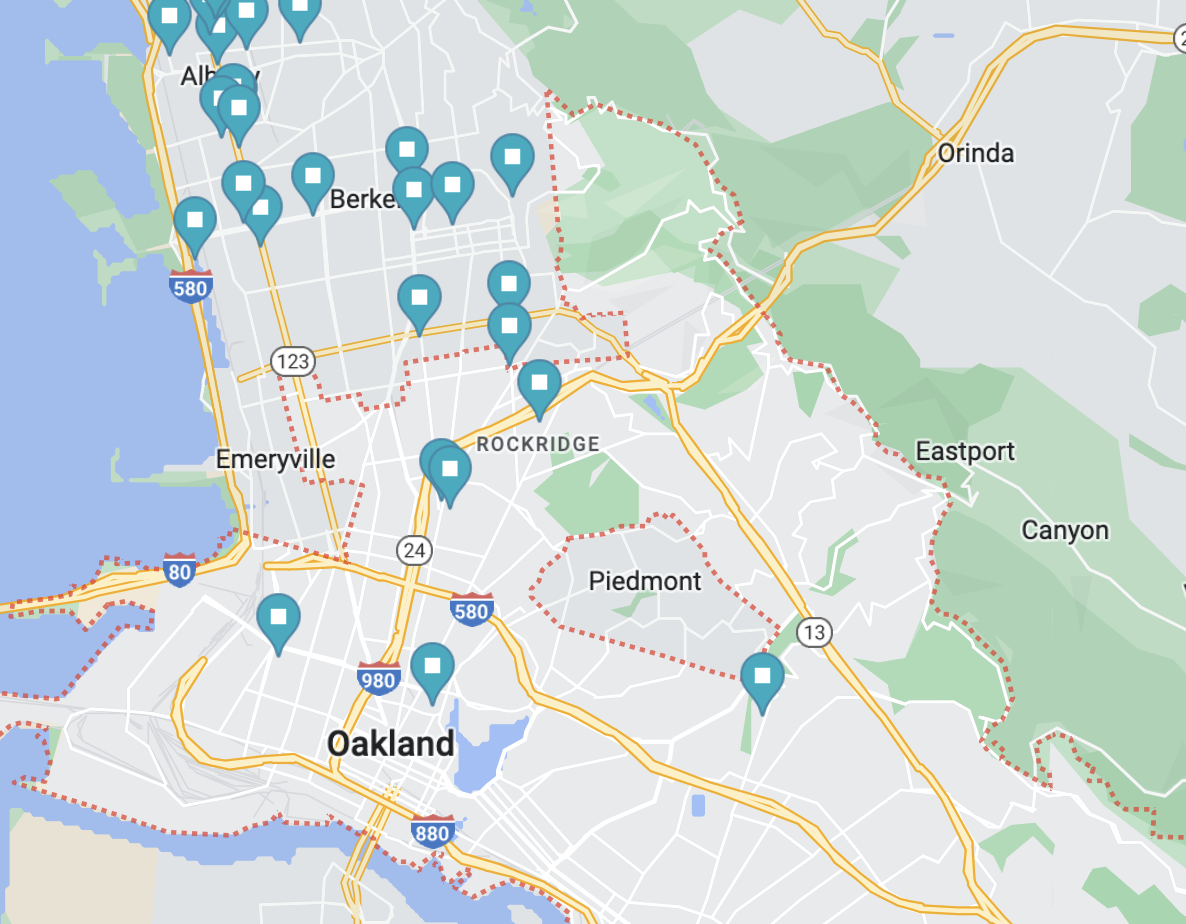
\includegraphics[width=0.7\textwidth]{figures/piedmont.png}
\end{frame}

\begin{frame}{Implementing regression discontinuity designs}

With a running variable $X$, an outcome $Y$, and a treatment $D$ allocated at the discontinuity, we estimate:

$$ Y_i = \alpha +  f(X_i) + \beta D_i + \varepsilon_i $$
    \begin{itemize}
        \item $f(X_i)$ is a smooth function of the running variable - e.g. just linear, or quadratic
        \item We could also estimate whether the \textbf{slope} changes at the discontinuity
        \item We are eventually interested in $\beta$: Does the outcome change at the discontinuity?
    \end{itemize}
\end{frame}



 \section{Broad topics for the exam}
 \begin{frame}{Introduction}
     \begin{itemize}
         \item Interpreting regression tables
         \item p-values: How surprised we should be to observe the world as it is if your hypothesis about how it works were true?
         \item Omitted variable bias
         \item Interpretation of control variables and their role
         \item Interaction terms (dummy or continuous) -- dummyXdummy: get means for every group
     \end{itemize}
 \end{frame}




  \begin{frame}{Instrumental variables}
     \begin{itemize}
         \item Calculation
         \item Three assumptions: Relevance, Independence (Exogeneity), Exclusion restriction
         \item Think of three regressions: First stage, reduced form, "target regression" (Second stage)
         \item Connection to RCTs (imperfect compliance)
         % \item Local Average Treatment Effect (ITT/TOT/\dots)
         % \item Connect with potential outcomes framework
     \end{itemize}
 \end{frame}


  \begin{frame}{Differences in Differences}
     \begin{itemize}
        % \item Connect with potential outcomes
         \item Parallel trends assumption
        \item Calculate with tables
        \item Calculate using regression tables 
     \end{itemize}
 \end{frame}


  \begin{frame}{Panel Data and Fixed effects}
     \begin{itemize}
         \item Fixed effects: Calculation
        % \item First-differences
         \item Useful way to think about it: We add a lot of controls, but key problem remains (time-varying confounders: Things that change over time that affect different units differently, e.g.: climate change ...)
         \item Connection of two-way fixed effects with DiD
     \end{itemize}
 \end{frame}


  \begin{frame}{Regression Discontinuities}
     \begin{itemize}
         \item "No jump but our jump at the jump"
         \item Fuzzy DiD is just IV
     \end{itemize}
 \end{frame}



  \begin{frame}{General and overarching concepts}
     \begin{itemize}
      %  \item Potential outcomes: Please review carefully -- maybe not on the long questions but who knows?
         \item Comparison of OLS and other estimates: What changed and why? (Hint: Always go back to OVB)%, less likely measurement error or reverse causality)
         \item Be \textbf{\alert{creative but also clear}}: Most thinking questions can be solved with reasonable economic intuition, your knowledge of the world, and what you learned on the course.
        \item Keep in mind the \textbf{\alert{big picture}}: We are just trying to find a valid counterfactual, to estimate causal effects! 
     \end{itemize}
 \end{frame}









\section{IV Exam Exercise}

\begin{frame}[allowframebreaks]{IV Exam exercise}
The land of Econometrea consists of 34 islands. Each island has their own university and students attend uni on their home island. Students in Econometrea either have to attend lectures in person or watch them online. Priyanka has obtained data for the students from all the universities and would like to study the effect of watching lectures online on the students’ exam scores. For each student she has the exam score (0 - 100, 70+ is a first, 40 and below a fail), which she uses as her left hand side variable, the fraction of lectures watched online, and how on how many days the student visited the library each week. Priyanka obtains the following regression results:\\

\framebreak 
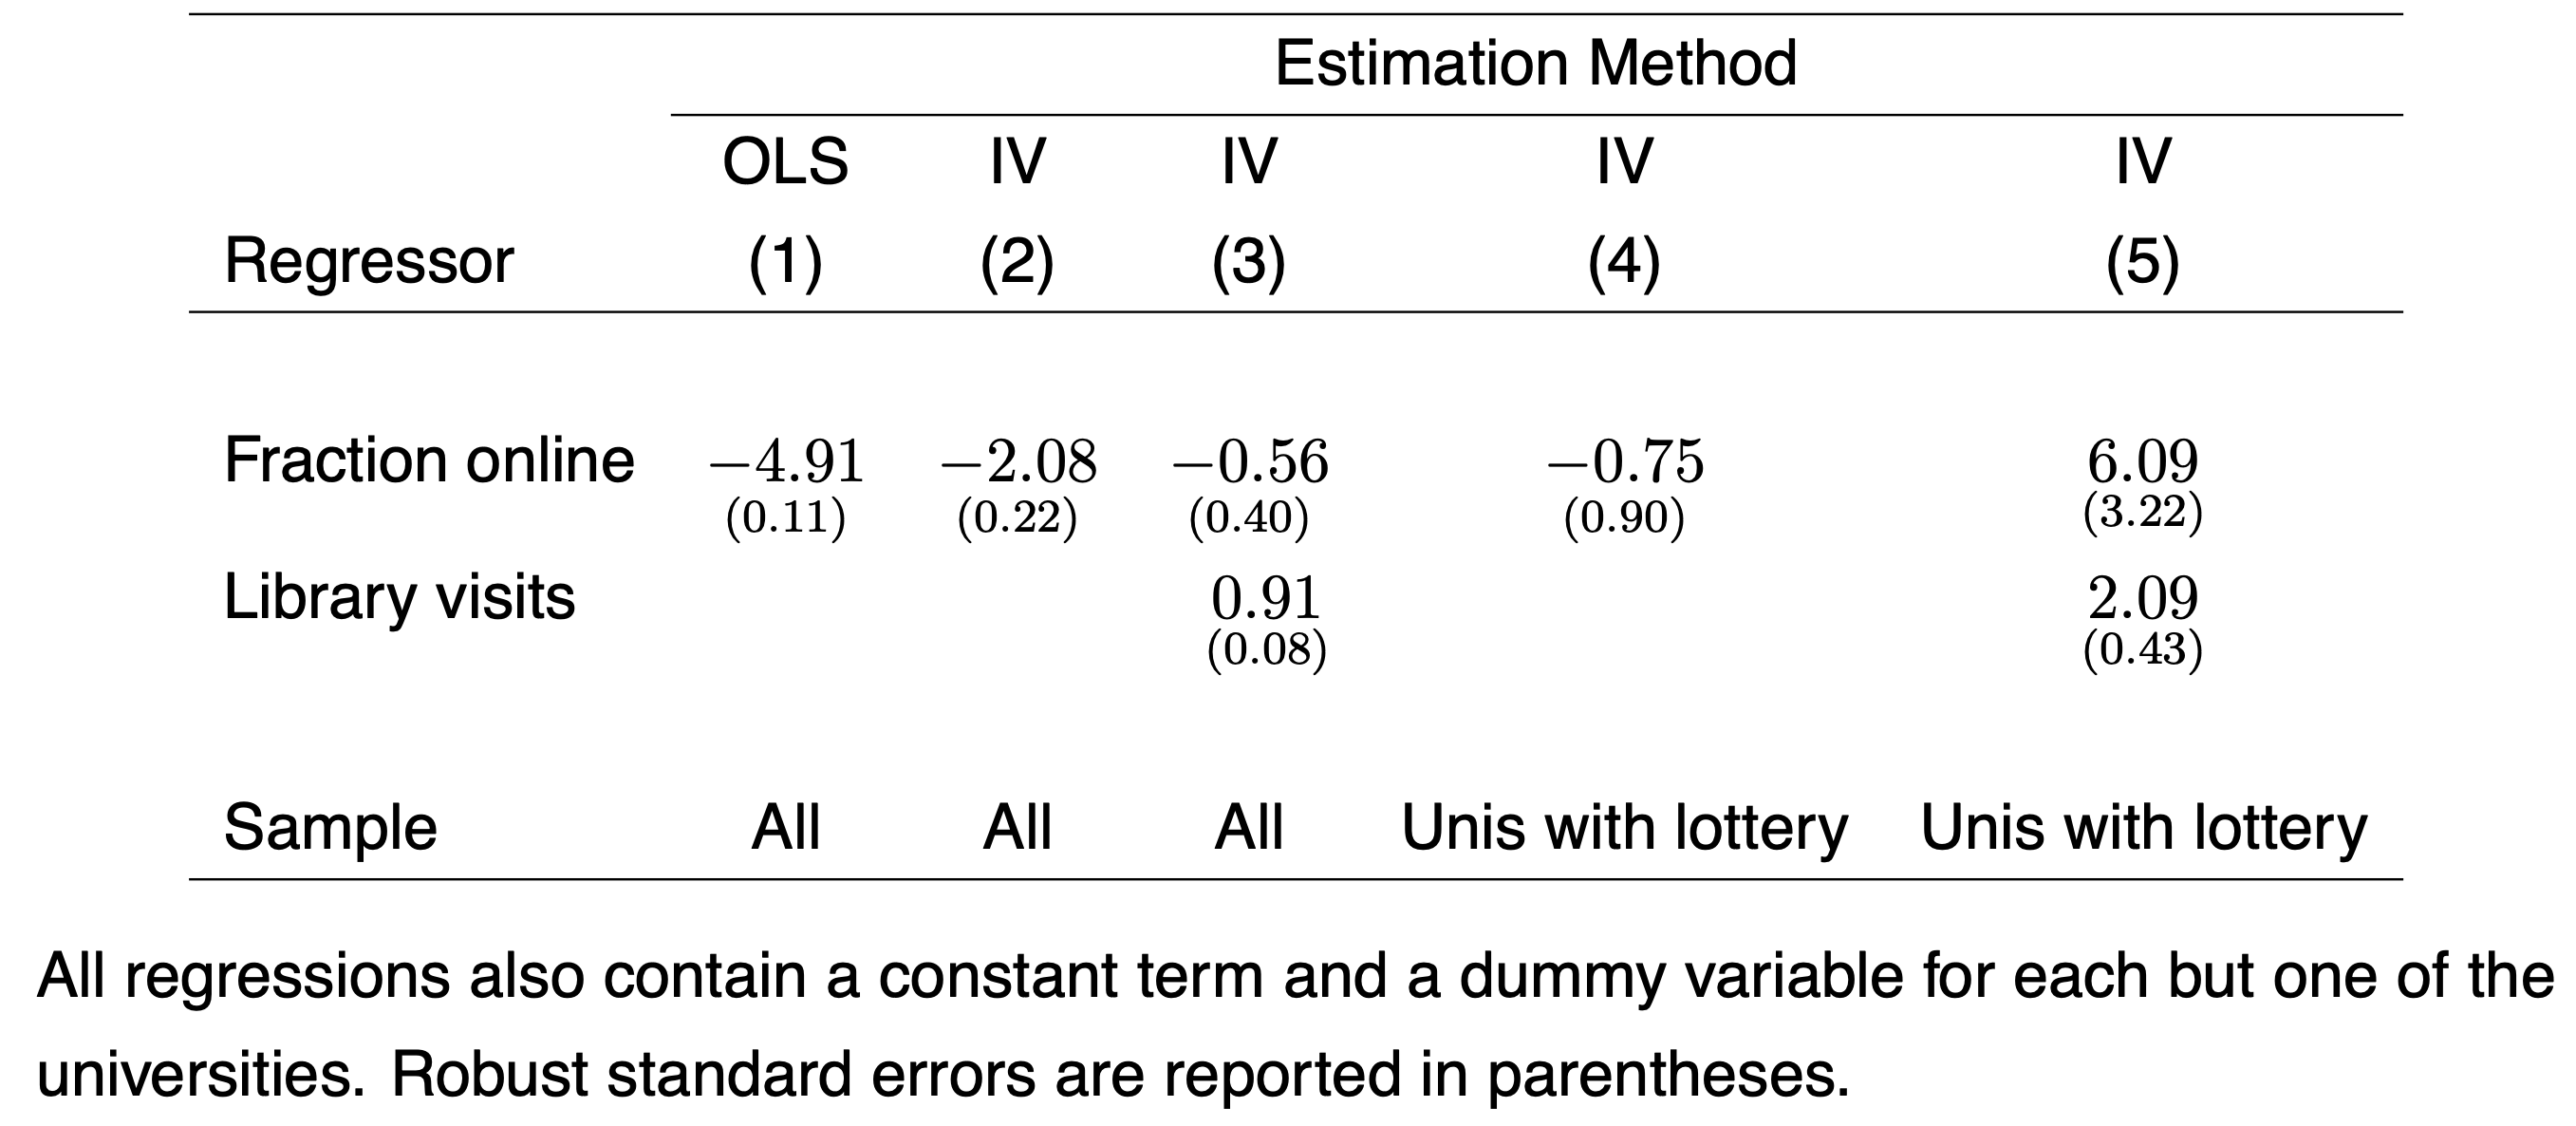
\includegraphics[width=1.0\textwidth]{tables/IV_Table.png}

\framebreak
(a) What is the interpretation of the coefficient in column (1). If this were a causal effect, would it be big or small? Explain whether this estimate is likely to have a causal interpretation.\\

(b) Your friend realizes that you also have data from before Covid, when all students had to attend all lectures in person. She suggests to construct a panel dataset and to run a regression and to include time and individual fixed effects. What assumption would be required for this regression to deliver a causal effect?

\framebreak
\alert{Solution}
\begin{itemize}
    \item Students who watch all lectures online, on average, have around 4.9 fewer points on the exam than students who went to all lecturs in person. This is a moderately strong effect, but likely not causal (think of omitted variables, such as student motivation)
\end{itemize}
\framebreak


\alert{Solution}
\begin{itemize}
    \item For this to work, we need the parallel assumption to hold: In the absence of Covid and the introduction of the online policy, individuals with more online attendance would have had the same change in exam scores as individuals with less online attendance. \\ 
    In this case, this might not be very plausible, because Covid probably affected individuals who are likely to stay at home differently than individuals who attend class in person.

\end{itemize}
\framebreak



\framebreak 
\small{
(c) Wei Min observes that some halls of residence are close to the lecture rooms while others are further away and suggests to use the distance of halls from lecture halls as an instrumental variable for the fraction of lectures watched online. Results are in column (2). Explain which assumptions need to be satisfied for the IV to deliver better causal estimates than OLS here. Discuss the validity of the assumptions in this case.}


\framebreak 
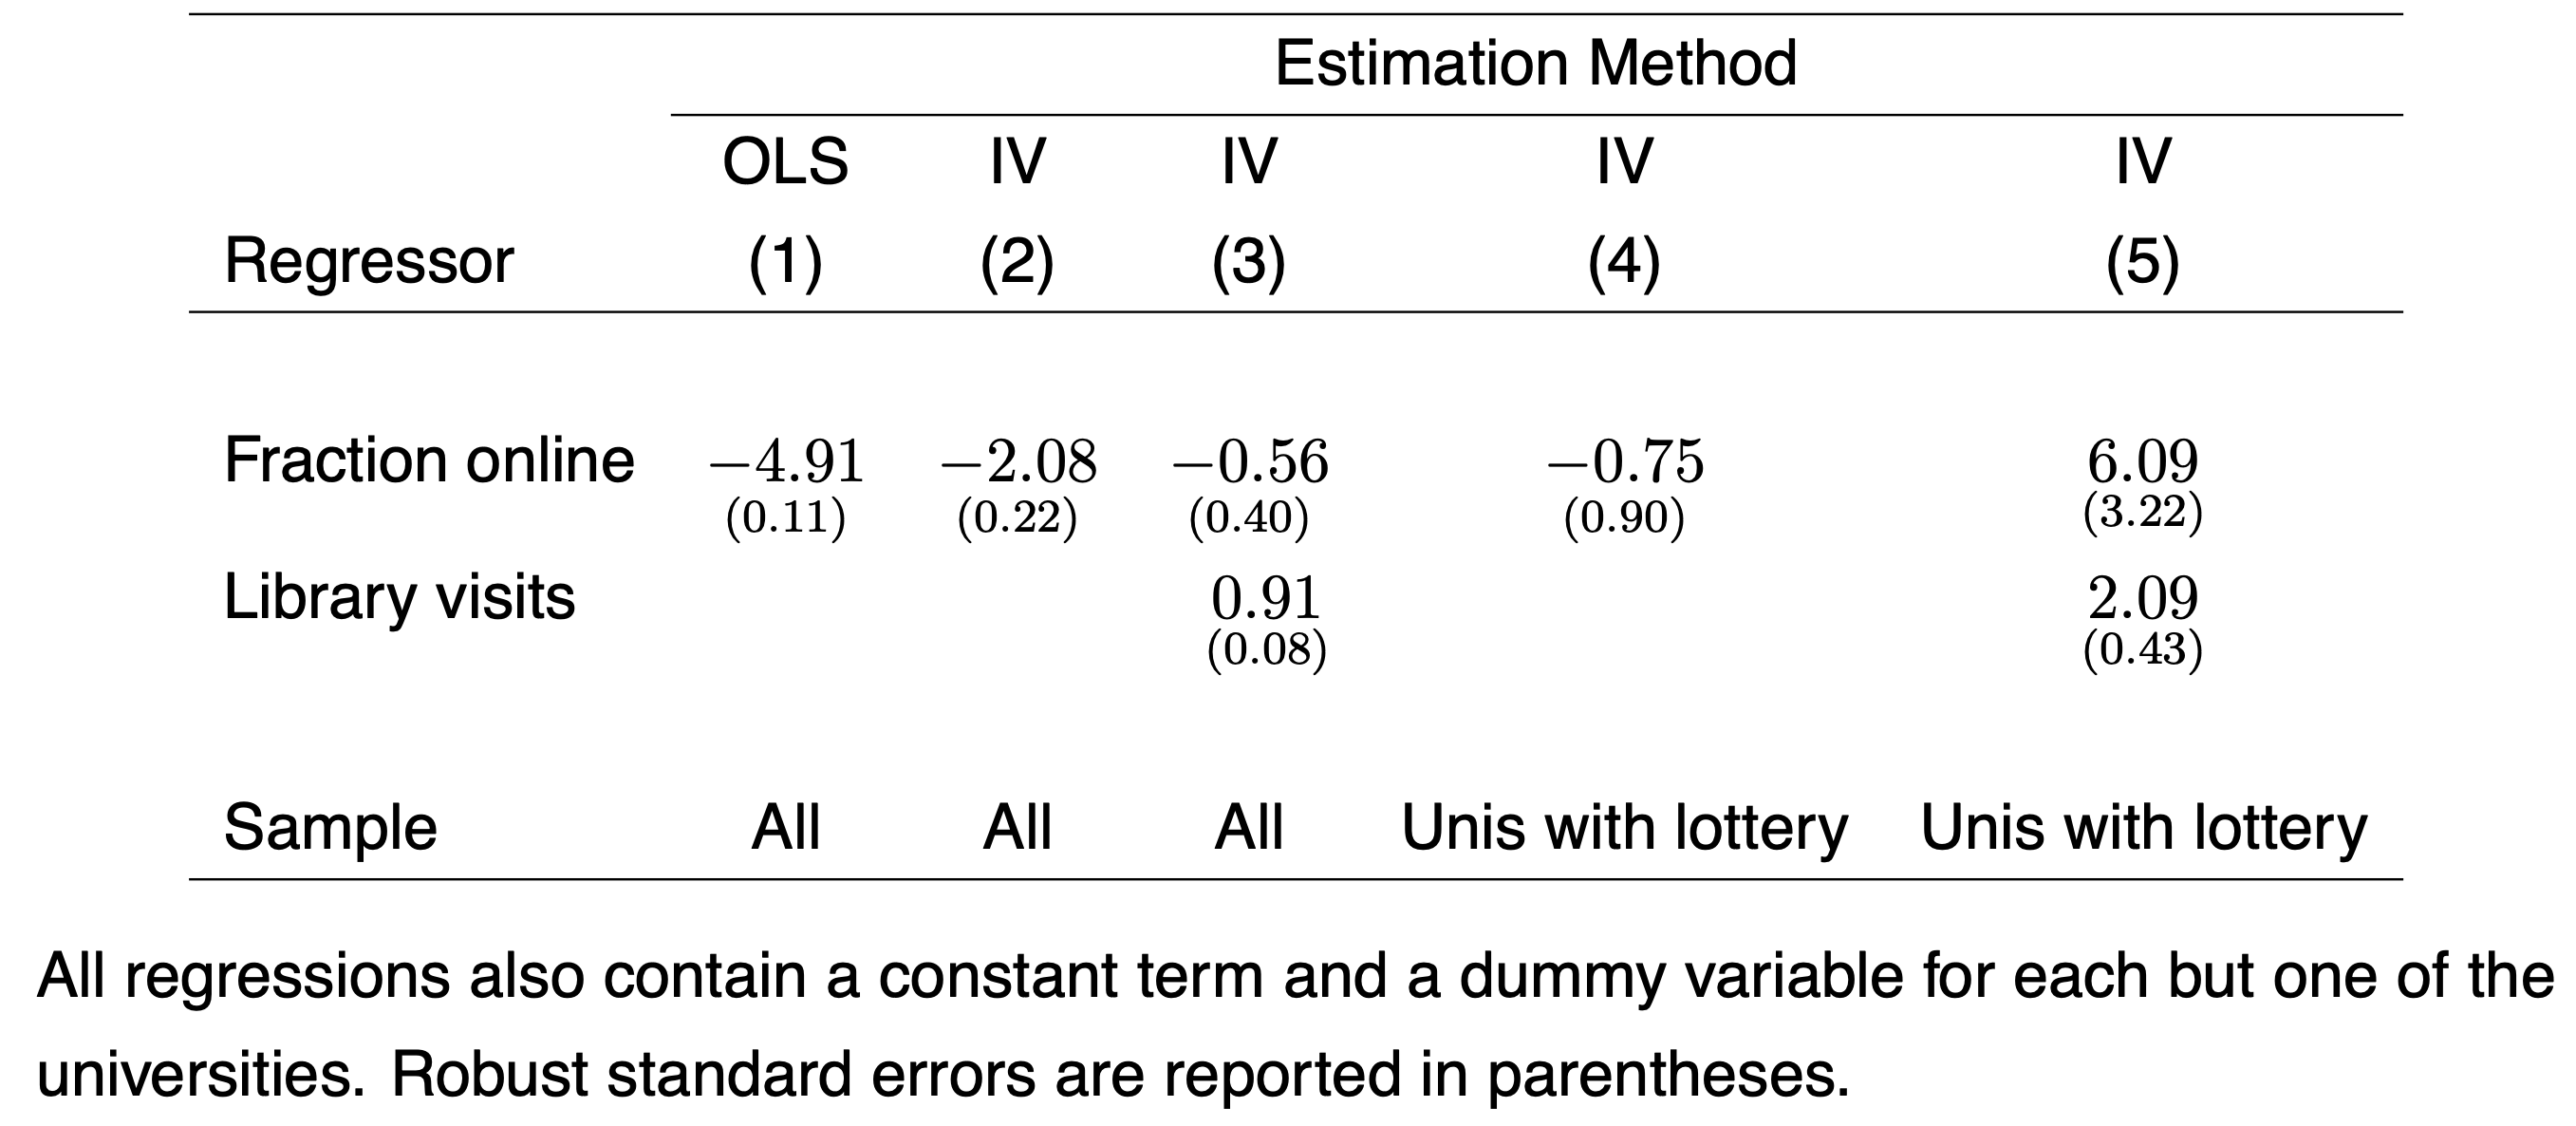
\includegraphics[width=0.9\textwidth]{tables/IV_Table.png}
\framebreak



\alert{Solution}
    \begin{itemize}
    \item \textbf{Relevance:} Proximity to lecture halls must correlate strongly with lecture attendance. This is plausible from our experience, and we could test this using an F-test.
    \item  
    \textbf{Independence/Exogeneity:}  Proximity must be as good as randomly allocated. This might not hold here, for example, if more motivated students live closer to campus.
    \item
    \textbf{Exclusion restruction:} Proximity to lecture halls only influences exam scores because it has an effect on lecture attendance. This can be violated if proximity also affects the probability to go and study in the library, or if residence halls closer to campus are also closer to bars
\end{itemize}

\framebreak
(d) Alma points out to Wei Min that students can pick which hall they want to live in and that some halls are located in Study Village, close to lecture halls and the library while others are located further away in Party Town, surrounded by pubs. How does this information affect your assessment of the IV strategy?\\
(e) Manuel realises that the data also include a variable for the number of times a student has checked into the library per week. He suggests to rerun the instrumental variables regression adding this variable as a control. Results for this regression are displayed in column (3). Assess Manuel’s strategy.

\framebreak 
\alert{Solution}
\begin{itemize}
    \item This would be a violation of independence/exogeneity: The students who live closer to the campus are just inherently different than students who live far away
    \item Library visits are a bad control: They are another outcome of the instrument, and so controlling for them introduces additional bias.
\end{itemize}

\framebreak 
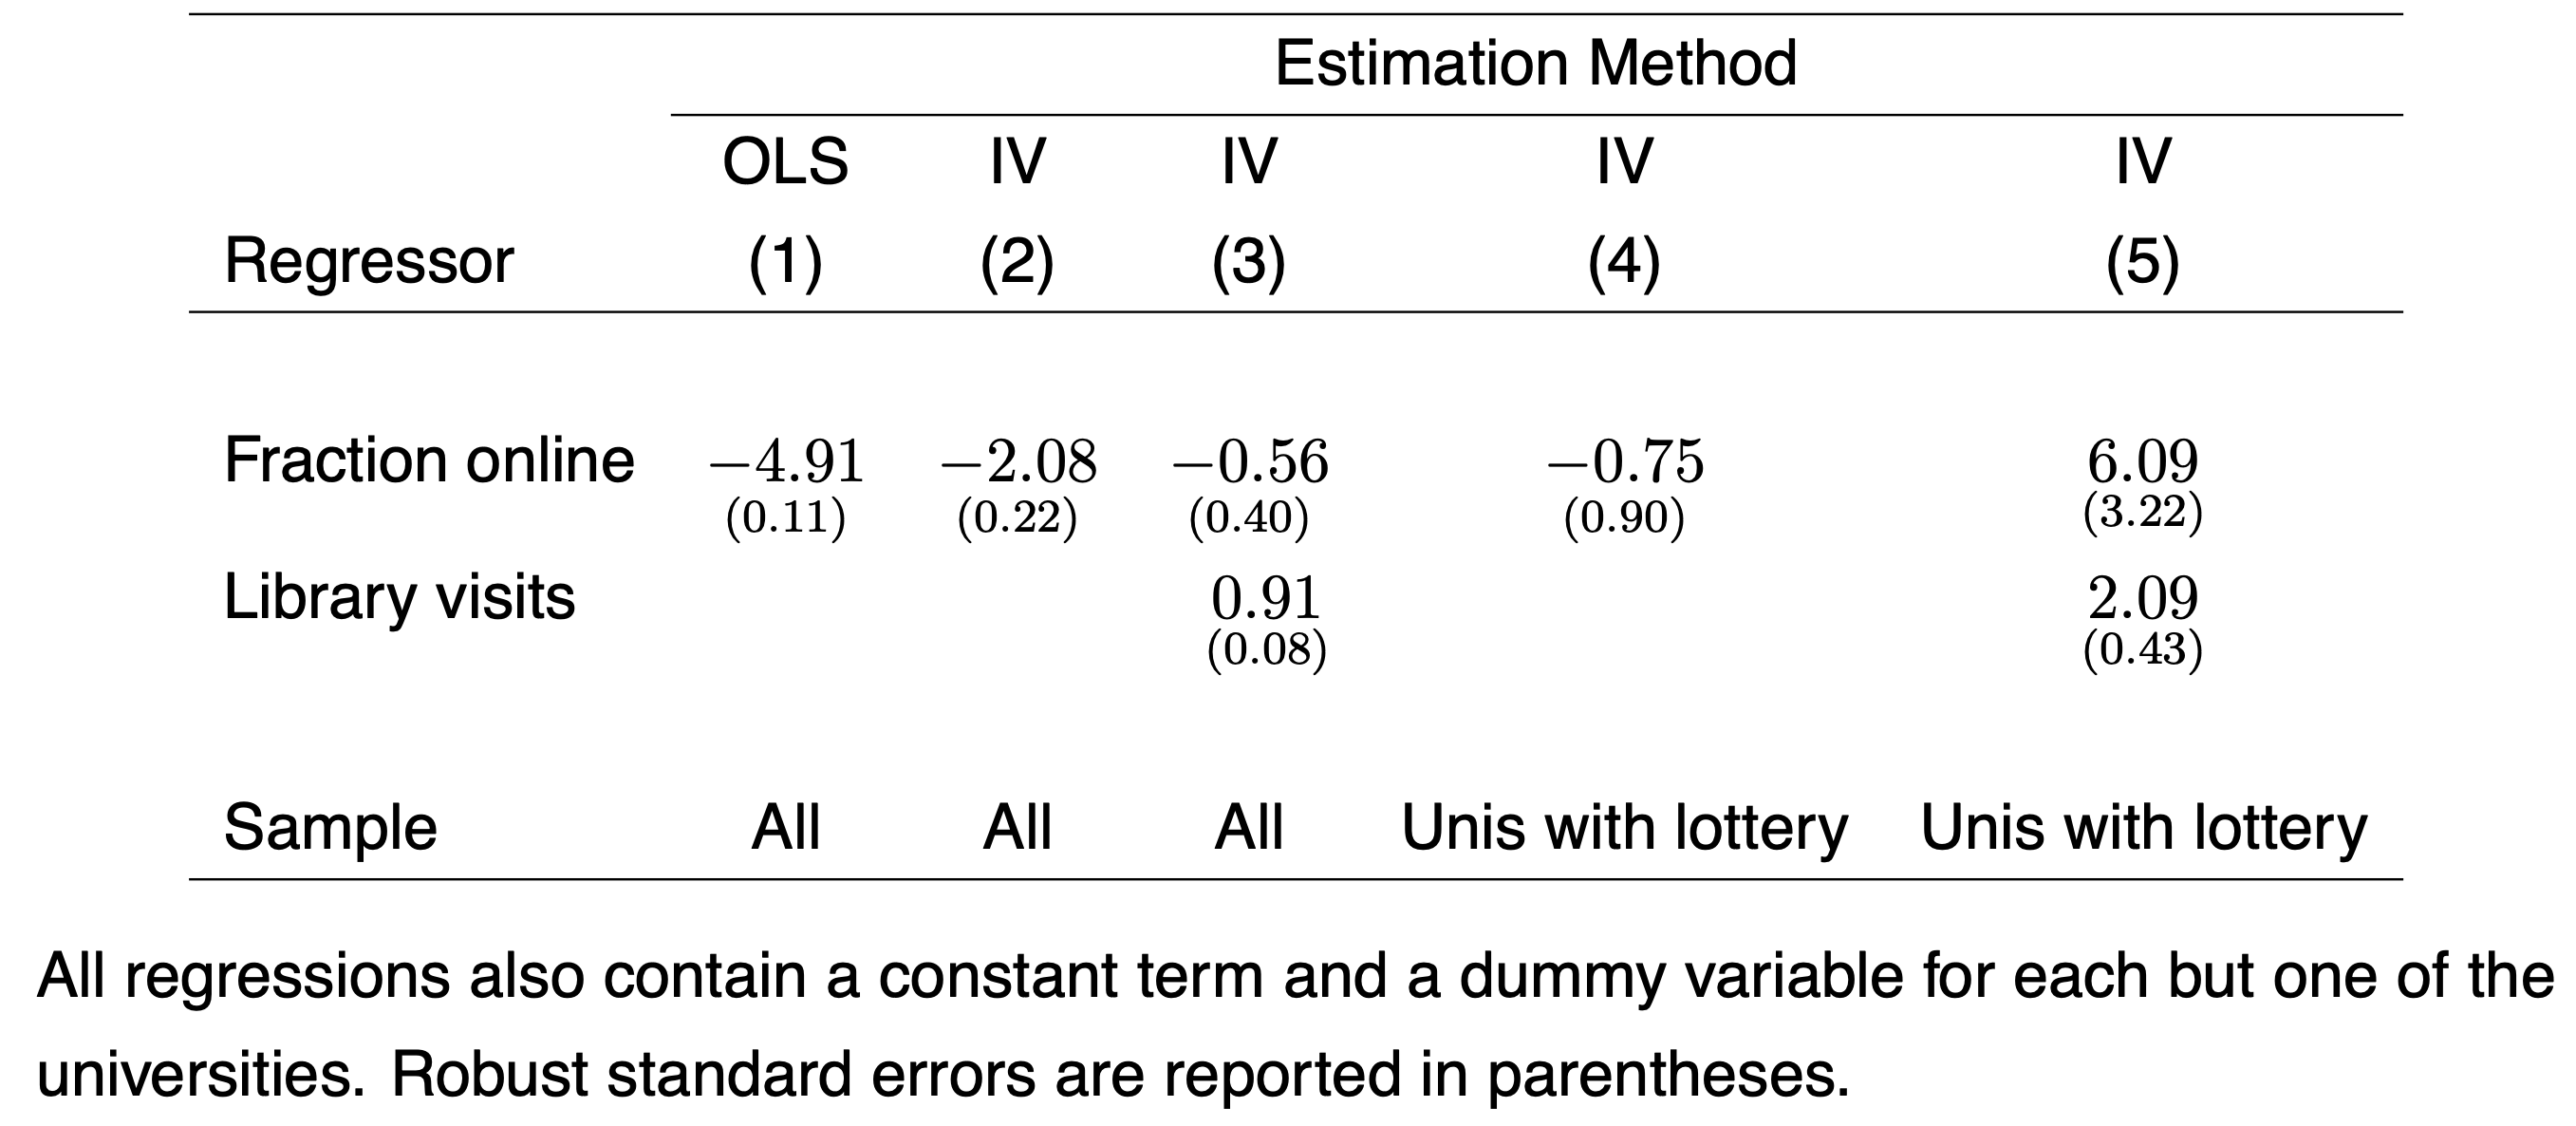
\includegraphics[width=1.0\textwidth]{tables/IV_Table.png}

\framebreak 


(f) Jenny notices that there are five universities which assign students to their halls of residence by a lottery. She suggests to run the IV model from columns (2) and (3) for the subsample of students from these universities only. Results are displayed in columns (4) and (5). Assess Jenny’s regressions.\\

(g) Drawing on the results in the table above, what have you learned from this exercise about the causal effect of watching lectures online on students’ exam results?


\framebreak 
\alert{Solution}
\begin{itemize}
    \item For these universities, the distance is as good as randomly assigned, and so we have no violations of the independence/exogeneity restriction. However, the exclusion restriction may still not hold.
    \item In a simply OLS regression, it may look as if watching lectures online causes worse grades. However, we can correct for this using a valid IV, and find that the effect is only very small and statistically insignificant.
\end{itemize}


\end{frame}





\section{Other exam practice}

\begin{frame}{RDD question}

    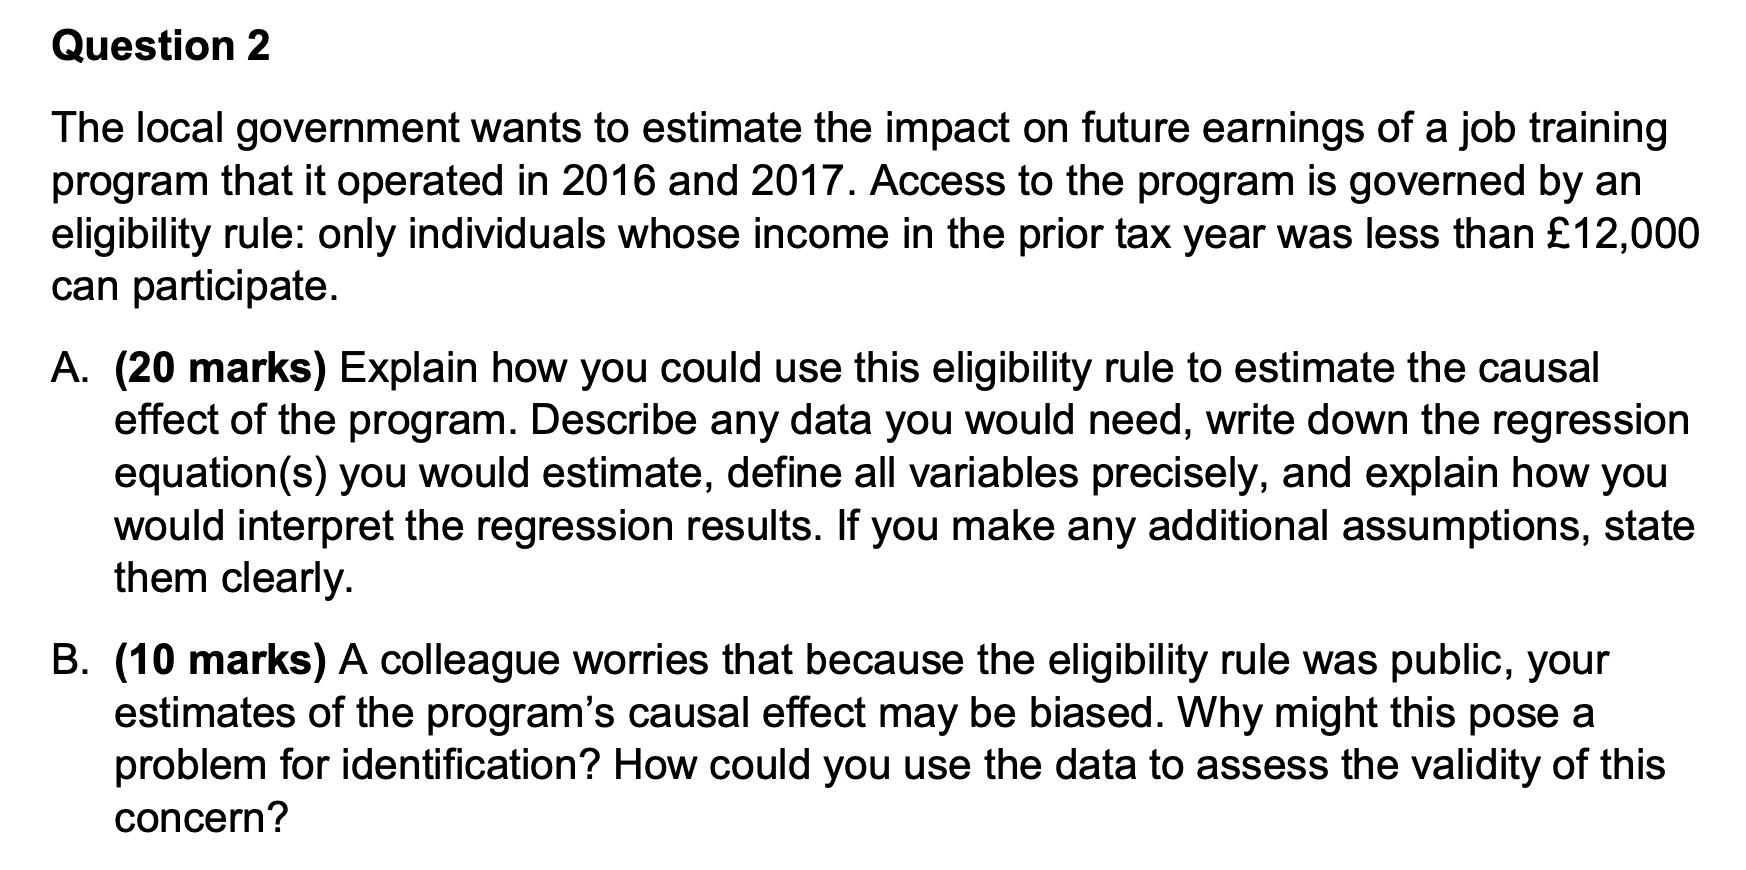
\includegraphics[width=1.0\textwidth]{figures/q_rdd_1.png}
\end{frame}



\begin{frame}{DiD question}

    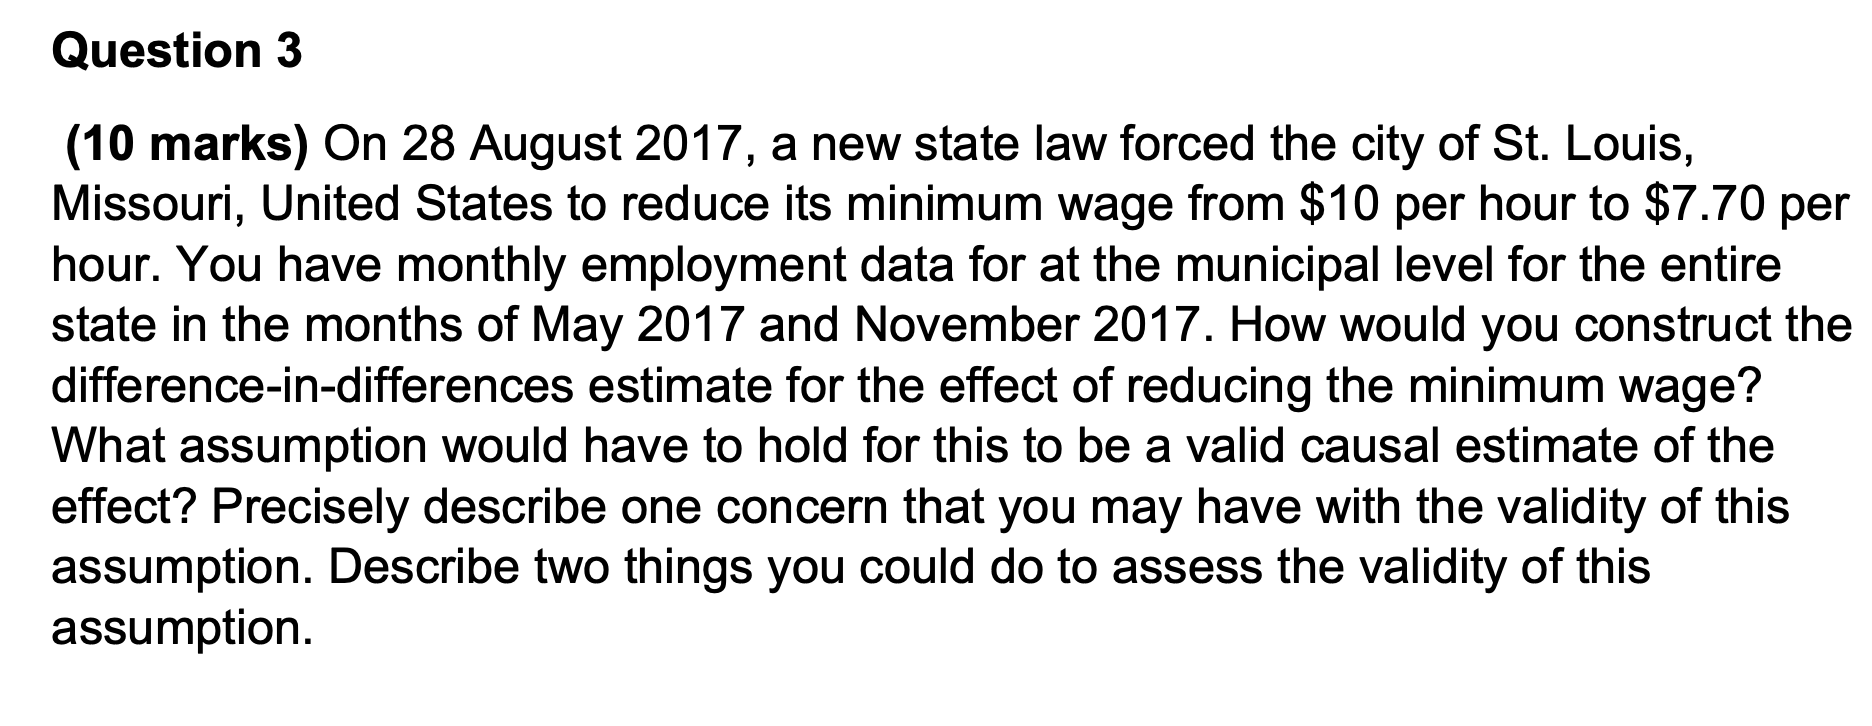
\includegraphics[width=1.0\textwidth]{figures/q_did.png}
\end{frame}






\end{document}
